Im Abschnitt \ref{sub:unterschiedeKameraUndMonitor} wurde bereits erklärt, dass die horizontalen Streifen in den Ergebnisbildern aus Abbildung \ref{img:minAndMaxLink} und Abbildung \ref{img:diffImage} hauptsächlich durch Unregelmäßigkeiten in dem Aufnahmeprozess entstehen.
Die Aufnahmeparameter bzw. Kameraeinstellungen müssen allerdings auf die Prüfstation und Prüfbedingungen angepasst werden, deshalb lassen sich diese horizontalen Streifen im Vorhinein nur begrenzt eliminieren.
Stattdessen kann man verschiedene Verfahren der Nachbearbeitung einsetzen.
Aufgrund der Periodizität und der festen Ausbreitungsrichtung der Streifen bietet es sich an, die Fourier-Analyse anzuwenden.
Man untersucht die Frequenzkomponenten der Streifen und filtert speziell diese aus dem Bild heraus, um sie zu entfernen.
Dennoch kann man so nicht die tatsächliche Information an den dunklen Streifen wiederherstellen, sondern lediglich eine Bildverbesserung durchführen.
Analog zur Überlegung aus Abschnitt \ref{sec:einsatzVonMehrerenStreifenmustern} ist eine andere Möglichkeit das Hinzuziehen von weiteren Bildern.
Da an den Stellen der horizontalen Streifen Informationen fehlen, kann man zusätzliche Muster zur Hand nehmen, um die Informationen zu ergänzen.
Man zieht weitere phasenverschobene Muster hinzu.
Um zu jedem Muster ein zugehöriges Muster mit einer Phasenverschiebung von $\pi$ zu haben, benötigt man eine gerade Anzahl an Mustern.
Wie auch in Abschnitt \ref{sec:einsatzVonMehrerenStreifenmustern} begründet, ist dies notwendig um die Oberflächeninformationen zu verknüpfen.
Dadurch eliminiert man Streifen, welche durch Überlappungen von Streifen in den unterschiedlichen Kamerabildern entstehen.

\p
Im Folgenden werden als Beispiel die vier Kamerabilder der Streifenmustern $m_1$ bis $m_4$ miteinander verknüpft, die mit $N_{shift} = 4$ gebildet wurden.
Aus den vier aufgenommenen Bildern verknüpft man je zwei Bilder mit der betragsmäßigen Differenz, in denen die Streifenmuster eine Phasenverschiebung von $\pi$ zueinander haben.
Die zwei resultierenden Bilder haben zueinander versetzte Streifen, die aus den Überlappungen entstehen.
Zum Schluss kann man die beiden Bilder so verknüpfen, dass man stets den Bildpunkt mit dem höheren Helligkeitswert nimmt.
Das entspricht der Maximierung.
Analog kann man auch die horizontalen Streifen aus Abbildung \ref{img:minAndMaxLink} eliminieren, in welcher die Typen von Fehlstellen isoliert voneinander betrachtet wurden.
In Abbildung \ref{img:imageTree} werden die einzelnen Schritte dieses Verfahrens veranschaulicht.

\begin{figure}[H]
	\centering
	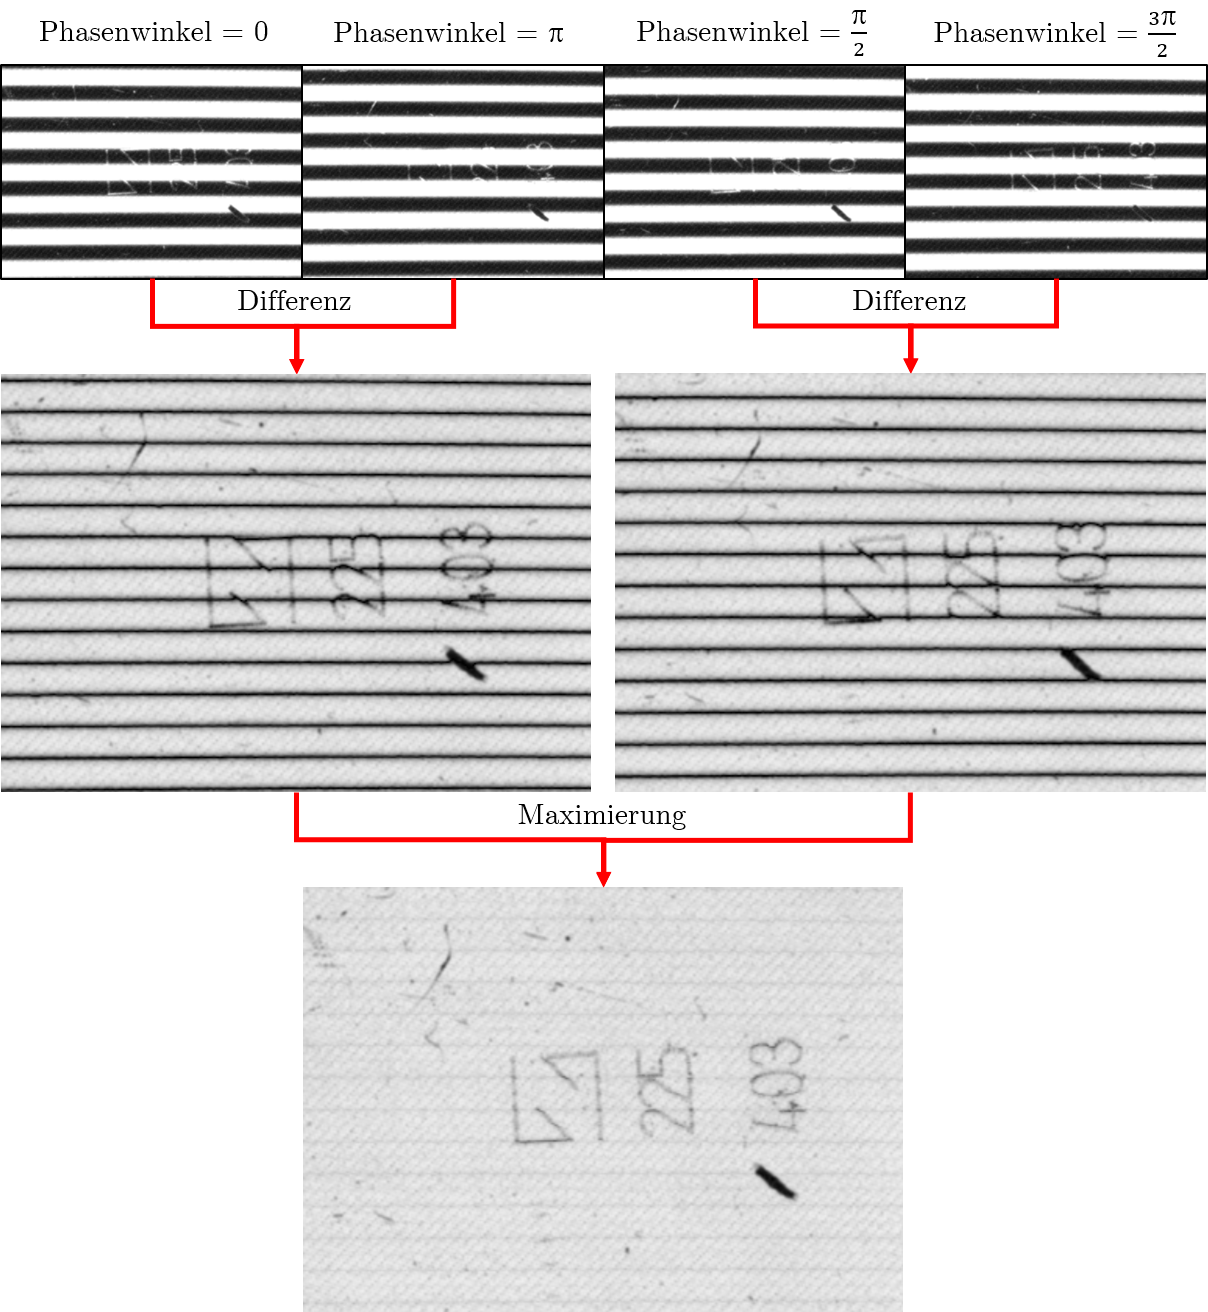
\includegraphics[width=\textwidth]{03_sichtpruefungDurchLichtstreuung/optimierungen/figures/imageTree}
	\caption[Prozess der Hervorhebung von Oberflächendefekten]{Prozess zur Hervorhebung von Oberflächendefekten mit $N_{shift} = 4$.}
	\label{img:imageTree}
\end{figure}

\noindent
Analog zu den gezeigten Schritten aus Abbildung \ref{img:imageTree} lässt sich auch die Verknüpfung von mehr als vier phasenverschobenen Streifenmustern durchführen.